\section{寄存器描述}
\regover{
{\hyperref[gpip-gpdac-config]{gpdac\_config}}&dac data control register
\\
\hline
{\hyperref[gpip-gpdac-dma-config]{gpdac\_dma\_config}}&dac dma control register
\\
\hline
{\hyperref[gpip-gpdac-dma-wdata]{gpdac\_dma\_wdata}}&dac fifo data register
\\
\hline
{\hyperref[gpip-gpdac-tx-fifo-status]{gpdac\_tx\_fifo\_status}}&dac status register
\\
\hline
{\hyperref[glb-dac-cfg0]{dac\_cfg0}}&DAC source control register
\\
\hline
{\hyperref[glb-dac-cfg1]{dac\_cfg1}}&DAC CHA control register
\\
\hline
{\hyperref[glb-dac-cfg2]{dac\_cfg2}}&DAC CHB control register
\\
\hline
{\hyperref[glb-dac-cfg3]{dac\_cfg3}}&DAC converter data register
\\
\hline
}

\subsection{gpadc\_config}
\label{gpip-gpadc-config}
地址:0x20002000
 \begin{figure}[H]
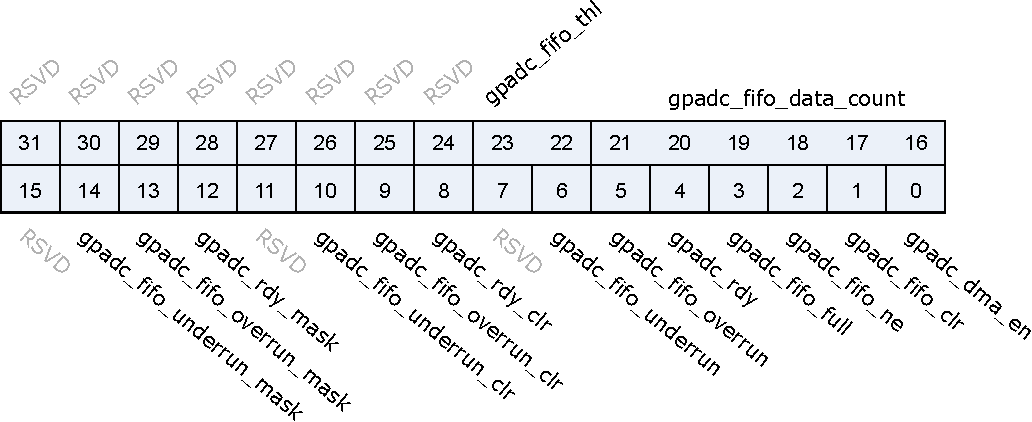
\includegraphics{gpip_gpadc_config.pdf}
\end{figure}

\regdes{31:24&RSVD& & & \\\hline
23:22&gpadc\_fifo\_thl&r/w&2'd0&fifo threshold \par 2'b00: 1 data  \par 2'b01: 4 data  \par 2'b10: 8 data \par 2'b11: 16 data
\\\hline
21:16&gpadc\_fifo\_data\_count&r&6'd0&fifo data number\\\hline
15&RSVD& & & \\\hline
14&gpadc\_fifo\_underrun\_mask&r/w&1'b0&write 1 mask\\\hline
13&gpadc\_fifo\_overrun\_mask&r/w&1'b0&write 1 mask\\\hline
12&gpadc\_rdy\_mask&r/w&1'b0&write 1 mask\\\hline
11&RSVD& & & \\\hline
10&gpadc\_fifo\_underrun\_clr&r/w&1'b0&Write 1 to clear flag\\\hline
9&gpadc\_fifo\_overrun\_clr&r/w&1'b0&Write 1 to clear flag\\\hline
8&gpadc\_rdy\_clr&r/w&1'b0&Write 1 to clear flag\\\hline
7&RSVD& & & \\\hline
6&gpadc\_fifo\_underrun&r&1'b0&FIFO underrun interrupt flag\\\hline
5&gpadc\_fifo\_overrun&r&1'b0&FIFO overrun interrupt flag\\\hline
4&gpadc\_rdy&r&1'b0&Conversion data ready interrupt flag\\\hline
3&gpadc\_fifo\_full&r&1'b0&FIFO full flag\\\hline
2&gpadc\_fifo\_ne&r&1'b0&FIFO not empty flag\\\hline
1&gpadc\_fifo\_clr&w1c&1'b0&FIFO clear signal\\\hline
0&gpadc\_dma\_en&r/w&1'b0&GPADC DMA enbale\\\hline

}
\subsection{gpadc\_dma\_rdata}
\label{gpip-gpadc-dma-rdata}
地址:0x20002004
 \begin{figure}[H]
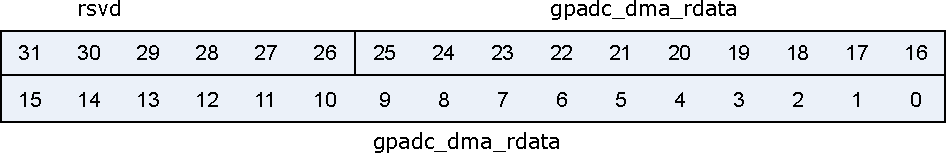
\includegraphics{gpip_gpadc_dma_rdata.pdf}
\end{figure}

\regdes{31:26&RSVD& & & \\\hline
25:0&gpadc\_dma\_rdata&r&26'd0&GPADC finial conversion result stored in the FIFO\\\hline

}
\subsection{gpdac\_config}
\label{gpip-gpdac-config}
地址:0x20002040
 \begin{figure}[H]
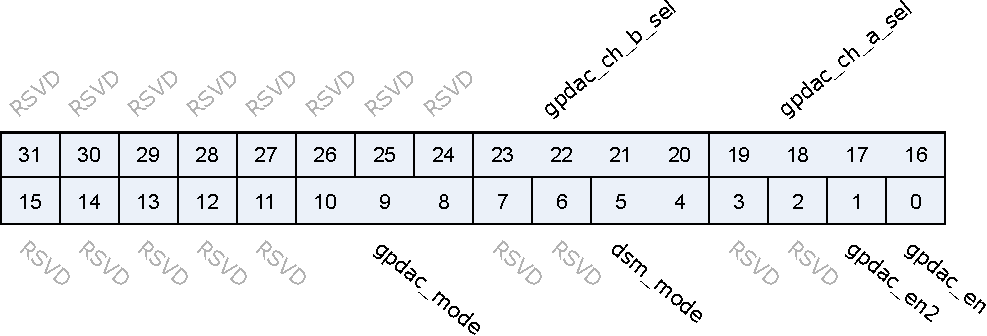
\includegraphics{gpip_gpdac_config.pdf}
\end{figure}

\regdes{31:24&RSVD& & & \\\hline
23:20&gpdac\_ch\_b\_sel&r/w&0&Channel B Source Select \par 0: Reg \par 1: DMA \par 3: Sin Gen \par 4: A (The same as channel A) \par 5: ~A (Inverse of channel A)
\\\hline
19:16&gpdac\_ch\_a\_sel&r/w&0&Channel A Source Select \par 0: Reg \par 1: DMA \par 3: Sin Gen
\\\hline
15:11&RSVD& & & \\\hline
10:8&gpdac\_mode&r/w&0&0:32k, 1:16k, 3:8k,  4:512k(for DMA only)\\\hline
7:1&RSVD& & & \\\hline
0&gpdac\_en&r/w&0&GPDAC enable\\\hline

}
\subsection{gpdac\_dma\_config}
\label{gpip-gpdac-dma-config}
地址:0x20002044
 \begin{figure}[H]
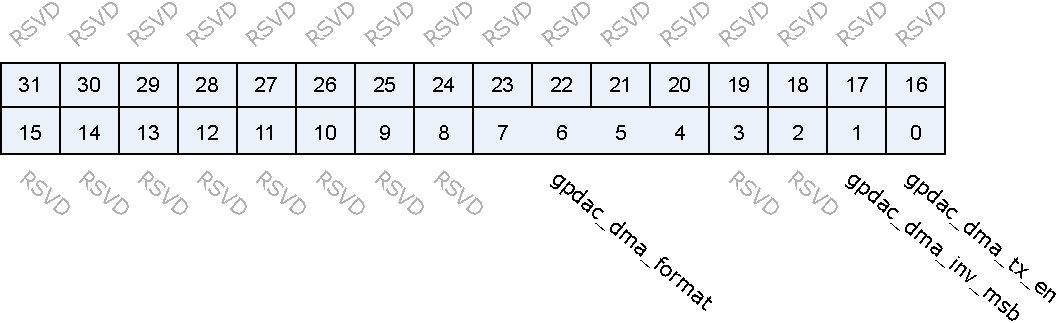
\includegraphics{gpip_gpdac_dma_config.pdf}
\end{figure}

\regdes{31:8&RSVD& & & \\\hline
7:4&gpdac\_dma\_format&r/w&0&DMA TX format (Data 12-bit) \par 0: ([11:0]) {A0}, {A1}, {A2}… \par 1: ([27:16][11:0]) {B0,A0}, {B1,A1}, {B2,A2}… \par 2: ([27:16][11:0]) {A1,A0}, {A3,A2}, {A5,A4}… \par 4: ([15:4]) {A0}, {A1}, {A2}… \par 5: ([31:20][15:4]) {B0,A0}, {B1,A1}, {B2,A2}… \par 6: ([31:20][15:4]) {A1,A0}, {A3,A2}, {A5,A4}… \par 8: ([31:24][23:16][15:8][7:0]) {A3,A2,A1,A0}, {A7,A6,A5,A4}… \par 9: ([31:24][23:16][15:8][7:0]) {B1,B0,A1,A0}, {B3,B2,A3,A2}… \par 10: ([31:24][23:16][15:8][7:0]) {B1,A1,B0,A0}, {B3,A3,B2,A2}… \par 11: ([15:8][7:0]) {B0,A0}, {B1,A1}, {B2,A2}…
\\\hline
3:2&RSVD& & & \\\hline
1&gpdac\_dma\_inv\_msb&r/w&0&GPDAC DMA Data Inverse MSB\\\hline
0&gpdac\_dma\_tx\_en&r/w&0&GPDAC DMA TX enable\\\hline

}
\subsection{gpdac\_dma\_wdata}
\label{gpip-gpdac-dma-wdata}
地址:0x20002048
 \begin{figure}[H]
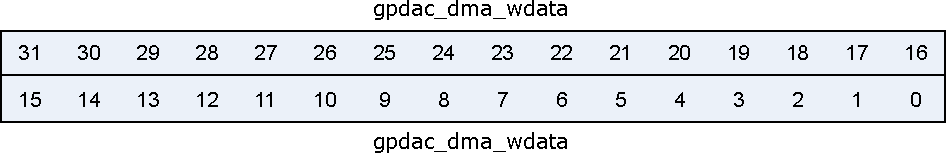
\includegraphics{gpip_gpdac_dma_wdata.pdf}
\end{figure}

\regdes{31:0&gpdac\_dma\_wdata&w&x&GPDAC DMA TX data\\\hline

}
\subsection{gpdac\_tx\_fifo\_status}
\label{gpip-gpdac-tx-fifo-status}
地址:0x2000204c
 \begin{figure}[H]
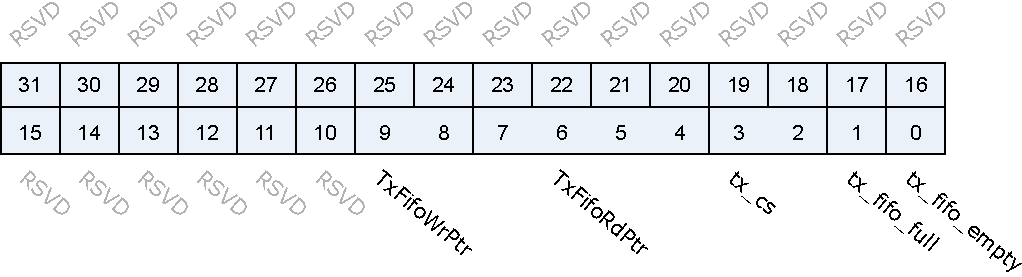
\includegraphics{gpip_gpdac_tx_fifo_status.pdf}
\end{figure}

\regdes{31:2&RSVD& & & \\\hline
1&tx\_fifo\_full&r&0&fifo full flag\\\hline
0&tx\_fifo\_empty&r&0&fifo empty flag\\\hline

}
\subsection{dac\_cfg0}
\label{glb-dac-cfg0}
地址:0x20000120
 \begin{figure}[H]
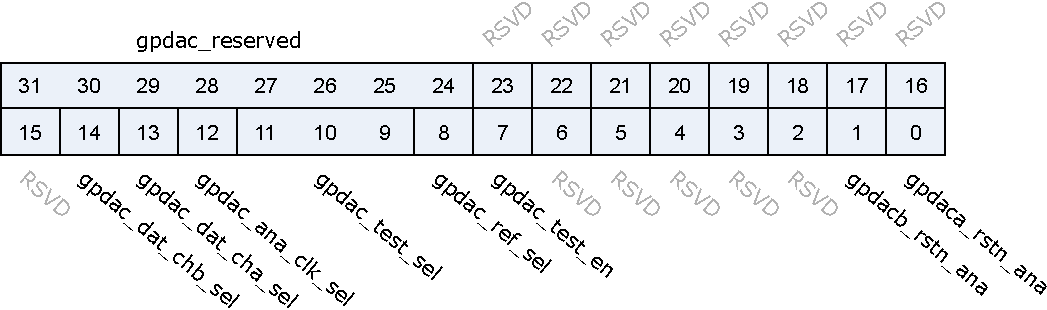
\includegraphics{glb_dac_cfg0.pdf}
\end{figure}

\regdes{31:15&RSVD& & & \\\hline
14&gpdac\_dat\_chb\_sel&r/w&1'h0&0:data from gpip, 1:data from audio pwm\\\hline
13&gpdac\_dat\_cha\_sel&r/w&1'h0&0:data from gpip, 1:data from audio pwm\\\hline
12&gpdac\_ana\_clk\_sel&r/w&1'h0&0:clock from gpip, 1:clock from audio pwm\\\hline
11:9&gpdac\_test\_sel&r/w&3'h0&select test point 0~7\\\hline
8&gpdac\_ref\_sel&r/w&1'h0&Reference select \par 1'h0 Internal reference \par 1'h1 External reference
\\\hline
7&gpdac\_test\_en&r/w&1'h0&Test enable 1'h0 analog test disabled (ATEST is set in Hi-Z state) 1'h1 analog test point enabled to ATEST\\\hline
6:2&RSVD& & & \\\hline
1&gpdacb\_rstn\_ana&r/w&1'h1&Soft reset for DAC channel B, active low\\\hline
0&gpdaca\_rstn\_ana&r/w&1'h1&Soft reset for DAC channel A, active low\\\hline

}
\subsection{dac\_cfg1}
\label{glb-dac-cfg1}
地址:0x20000124
 \begin{figure}[H]
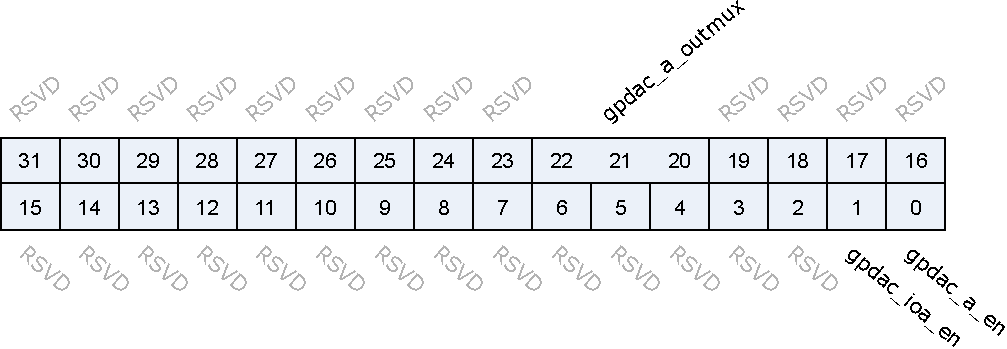
\includegraphics{glb_dac_cfg1.pdf}
\end{figure}

\regdes{31:20&RSVD& & & \\\hline
19:18&gpdac\_a\_rng&r/w&2'h3&Output voltage range control with internal/external reference\\\hline
17:2&RSVD& & & \\\hline
1&gpdac\_ioa\_en&r/w&1'h0&Channel A conversion output to pad enable \par 1'h0 Disable channel A conversion result to GPIO \par 1'h1 Enable channel A conversion result to GPIO
\\\hline
0&gpdac\_a\_en&r/w&1'h0&Channel A enable/disable signal \par 1'h0 Disable channel A conversion. \par 1'h1 Enable channel A conversion
\\\hline

}
\subsection{dac\_cfg2}
\label{glb-dac-cfg2}
地址:0x20000128
 \begin{figure}[H]
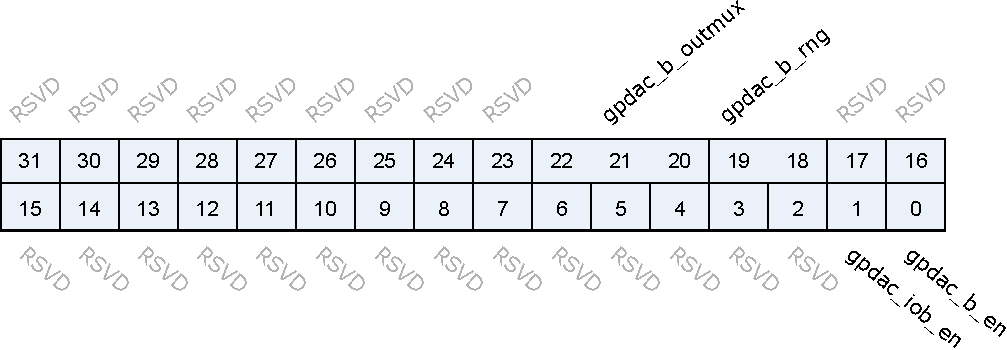
\includegraphics{glb_dac_cfg2.pdf}
\end{figure}

\regdes{31:20&RSVD& & & \\\hline
19:18&gpdac\_b\_rng&r/w&2'h3&Output voltage range control with internal/external reference\\\hline
17:2&RSVD& & & \\\hline
1&gpdac\_iob\_en&r/w&1'h0&channel B conversion output to pad enable \par 1'h0 Disable channel B conversion result to GPIO \par 1'h1 Enable channel B conversion result to GPIO
\\\hline
0&gpdac\_b\_en&r/w&1'h0&channel B enable/disable signal \par 1'h0 Disable channel B conversion. \par 1'h1 Enable channel B conversion
\\\hline

}
\subsection{dac\_cfg3}
\label{glb-dac-cfg3}
地址:0x2000012c
 \begin{figure}[H]
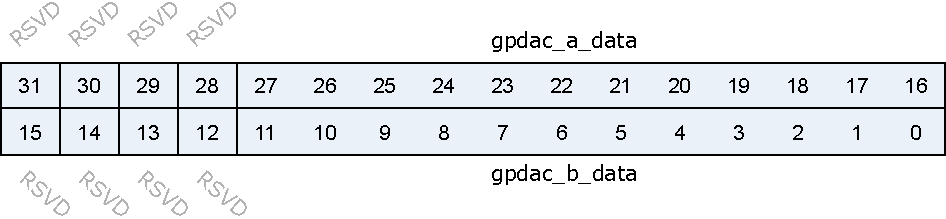
\includegraphics{glb_dac_cfg3.pdf}
\end{figure}

\regdes{31:28&RSVD& & & \\\hline
27:16&gpdac\_a\_data&r/w&12'h0&Channel A Data input\\\hline
15:12&RSVD& & & \\\hline
11:0&gpdac\_b\_data&r/w&12'h0&Channel B Data input\\\hline

}
